\documentclass[a4paper,12pt]{article}
\usepackage[utf8]{inputenc}
\usepackage[spanish]{babel}
\usepackage{color}
\usepackage{parskip}
\usepackage{graphicx}
\usepackage{multirow}
\usepackage{listings}
\usepackage{vmargin}
\usepackage{datetime}
\newdate{date}{16}{11}{2017}
\graphicspath{ {imagenes/} }
\definecolor{mygreen}{rgb}{0,0.6,0}
\definecolor{lbcolor}{rgb}{0.9,0.9,0.9}
\usepackage{epstopdf}
\usepackage{float}


\setpapersize{A4}
\setmargins{2.5cm}       % margen izquierdo
{1.5cm}                        % margen superior
{16.5cm}                      % anchura del texto
{23.42cm}                    % altura del texto
{10pt}                           % altura de los encabezados
{1cm}                           % espacio entre el texto y los encabezados
{0pt}                             % altura del pie de página
{2cm}     

\lstset{
    tabsize=4,    
%   rulecolor=,
    language=[GNU]C++,
        basicstyle=\tiny,
        aboveskip={1.5\baselineskip},
        columns=fixed,
        showstringspaces=false,
        extendedchars=false,
        breaklines=true,
        prebreak = \raisebox{0ex}[0ex][0ex]{\ensuremath{\hookleftarrow}},
        frame=single,
        showtabs=false,
        showspaces=false,
        showstringspaces=false,
        identifierstyle=\ttfamily,
        keywordstyle=\color[rgb]{0,0,1},
        commentstyle=\color[rgb]{0.026,0.112,0.095},
        stringstyle=\color{red},
        numberstyle=\color[rgb]{0.205, 0.142, 0.73},
%        \lstdefinestyle{C++}{language=C++,style=numbers}’.
}


\begin{document}
\title{Práctica de Laboratorio 5}
\author{
Christofer Fabián Chávez Carazas \\
\small{Universidad Nacional de San Agustín de Arequipa} \\
\small{Escuela Profesional de Ciencia de la Computación} \\
\small{Computación Gráfica}
}
\date{\displaydate{date}}

\maketitle

\begin{enumerate}
 \item \textbf{Desarrollar un programa para mostrar las primitivas de OpenGL}
 
 \begin{lstlisting}
#include <GL/glut.h>
#include <iostream>

using namespace std;

GLsizei winWidth = 1200, winHeight = 800;
int primitiva = -1;

enum Primitivas {POINTS = 1, LINES, STRIP, LINE_LOOP, POLYGON, TRIANGLE_STRIP, TRIANGLES, TRIANGLE_FAN, QUADS, QUAD_STRIP};

void init(void){
    glClearColor(1.0,1.0,1.0,1.0);
    glMatrixMode(GL_PROJECTION);
    gluOrtho2D(0.0, 1200.0, 0.0, 800.0);
}

void drawString(string s, int x, int y){
	glColor3f(0.0, 0.0, 0.0);
	glRasterPos2i(x,y);
	for(char c : s){
		glutBitmapCharacter(GLUT_BITMAP_HELVETICA_12,c);
	}
	glColor3f(1.0, 0.0, 0.0);
}

void display(void){
	glClear(GL_COLOR_BUFFER_BIT);
    glColor3f(1.0, 0.0, 0.0);
    glPointSize(5);
    glBegin(GL_POINTS);
    	glVertex2i(70,770);
    	glVertex2i(90,770);
    	glVertex2i(80,750);
    	glVertex2i(90,760);
    glEnd();
    drawString("GL_POINTS", 50, 730);
    glBegin(GL_LINES);
    	glVertex2i(200, 730);
    	glVertex2i(250, 800);
    	glVertex2i(240, 760);
    	glVertex2i(270, 730);
    glEnd();
    drawString("GL_LINES", 205, 700);
    glBegin(GL_LINE_STRIP);
    	glVertex2i(500, 700);
    	glVertex2i(400, 780);
    	glVertex2i(350, 740);
    	glVertex2i(600, 760);
    	glVertex2i(500, 780);
    	glVertex2i(560, 670);
    	glVertex2i(450, 650);
    glEnd();
    drawString("GL_LINE_STRIP", 450, 620);
    glBegin(GL_LINE_LOOP);
    	glVertex2i(700, 750);
    	glVertex2i(800, 790);
    	glVertex2i(750, 780);
    	glVertex2i(750, 730);
    	glVertex2i(790, 720);
    	glVertex2i(740, 670);
    glEnd();
    drawString("GL_LINE_LOOP", 700, 640);
    glBegin(GL_POLYGON);
    	glVertex2i(900, 750);
    	glVertex2i(950, 800);
    	glVertex2i(1000, 750);
    	glVertex2i(1000, 700);
    	glVertex2i(950, 650);
    	glVertex2i(900, 700);
    glEnd();
    drawString("GL_POLYGON", 910, 620);
    glBegin(GL_TRIANGLE_STRIP);
    	glVertex2i(100, 550);
    	glVertex2i(250, 540);
    	glVertex2i(130, 450);
    	glColor3f(0.0, 1.0, 0.0);
    	glVertex2i(220, 460);
    	glVertex2i(110, 400);
    	glColor3f(0.0, 0.0, 1.0);
    	glVertex2i(210, 390);
    	glVertex2i(150, 350);
    	glColor3f(0.0, 0.0, 0.0);
    	glVertex2i(220, 360);
    glEnd();
    drawString("GL_TRIANGLE_STRIP", 120, 320);
    glBegin(GL_TRIANGLES);
    	glVertex2i(350, 500);
    	glVertex2i(400, 550);
    	glVertex2i(420, 490);
    	glVertex2i(460, 470);
    	glVertex2i(480, 520);
    	glVertex2i(550, 470);
    glEnd();
    drawString("GL_TRIANGLES", 390, 450);
    glBegin(GL_TRIANGLE_FAN);
    	glVertex2i(400, 340);
    	glVertex2i(420, 400);
    	glVertex2i(500, 405);
    	glColor3f(0.0, 1.0, 0.0);
    	glVertex2i(520, 370);
    	glColor3f(0.0, 0.0, 1.0);
    	glVertex2i(570, 350);
    	glColor3f(0.0, 0.0, 0.0);
    	glVertex2i(520, 320);
    glEnd();
    drawString("GL_TRIANGLE_FAN", 400, 300);
    glBegin(GL_QUADS);
    	glVertex2i(650, 520);
    	glVertex2i(660, 570);
    	glVertex2i(720, 550);
    	glVertex2i(690, 500);
    	glVertex2i(650, 450);
    	glVertex2i(730, 450);
    	glVertex2i(720, 420);
    	glVertex2i(630, 380);
    glEnd();
    drawString("GL_QUADS", 650, 350);
    glBegin(GL_QUAD_STRIP);
    	glVertex2i(800, 570);
    	glVertex2i(900, 580);
    	glVertex2i(820, 500);
    	glVertex2i(880, 510);
    	glColor3f(0.0, 1.0, 0.0);
    	glVertex2i(810, 460);
    	glVertex2i(875, 440);
    	glColor3f(0.0, 0.0, 1.0);
    	glVertex2i(850, 400);
    	glVertex2i(900, 420);
    glEnd();
    drawString("GL_QUAD_STRIP", 800, 380);

    glFlush();
}

int main(int argc, char **argv){
    glutInit(&argc, argv);
    glutInitDisplayMode(GLUT_SINGLE | GLUT_RGB);
    glutInitWindowSize(winWidth, winHeight);
    glutInitWindowPosition(100, 100);
    glutCreateWindow("Programa Primitivas");
    init();
    glutDisplayFunc(display);


    glutMainLoop();
    return 0;
}
\end{lstlisting}

\begin{figure}[H]
 \centering
 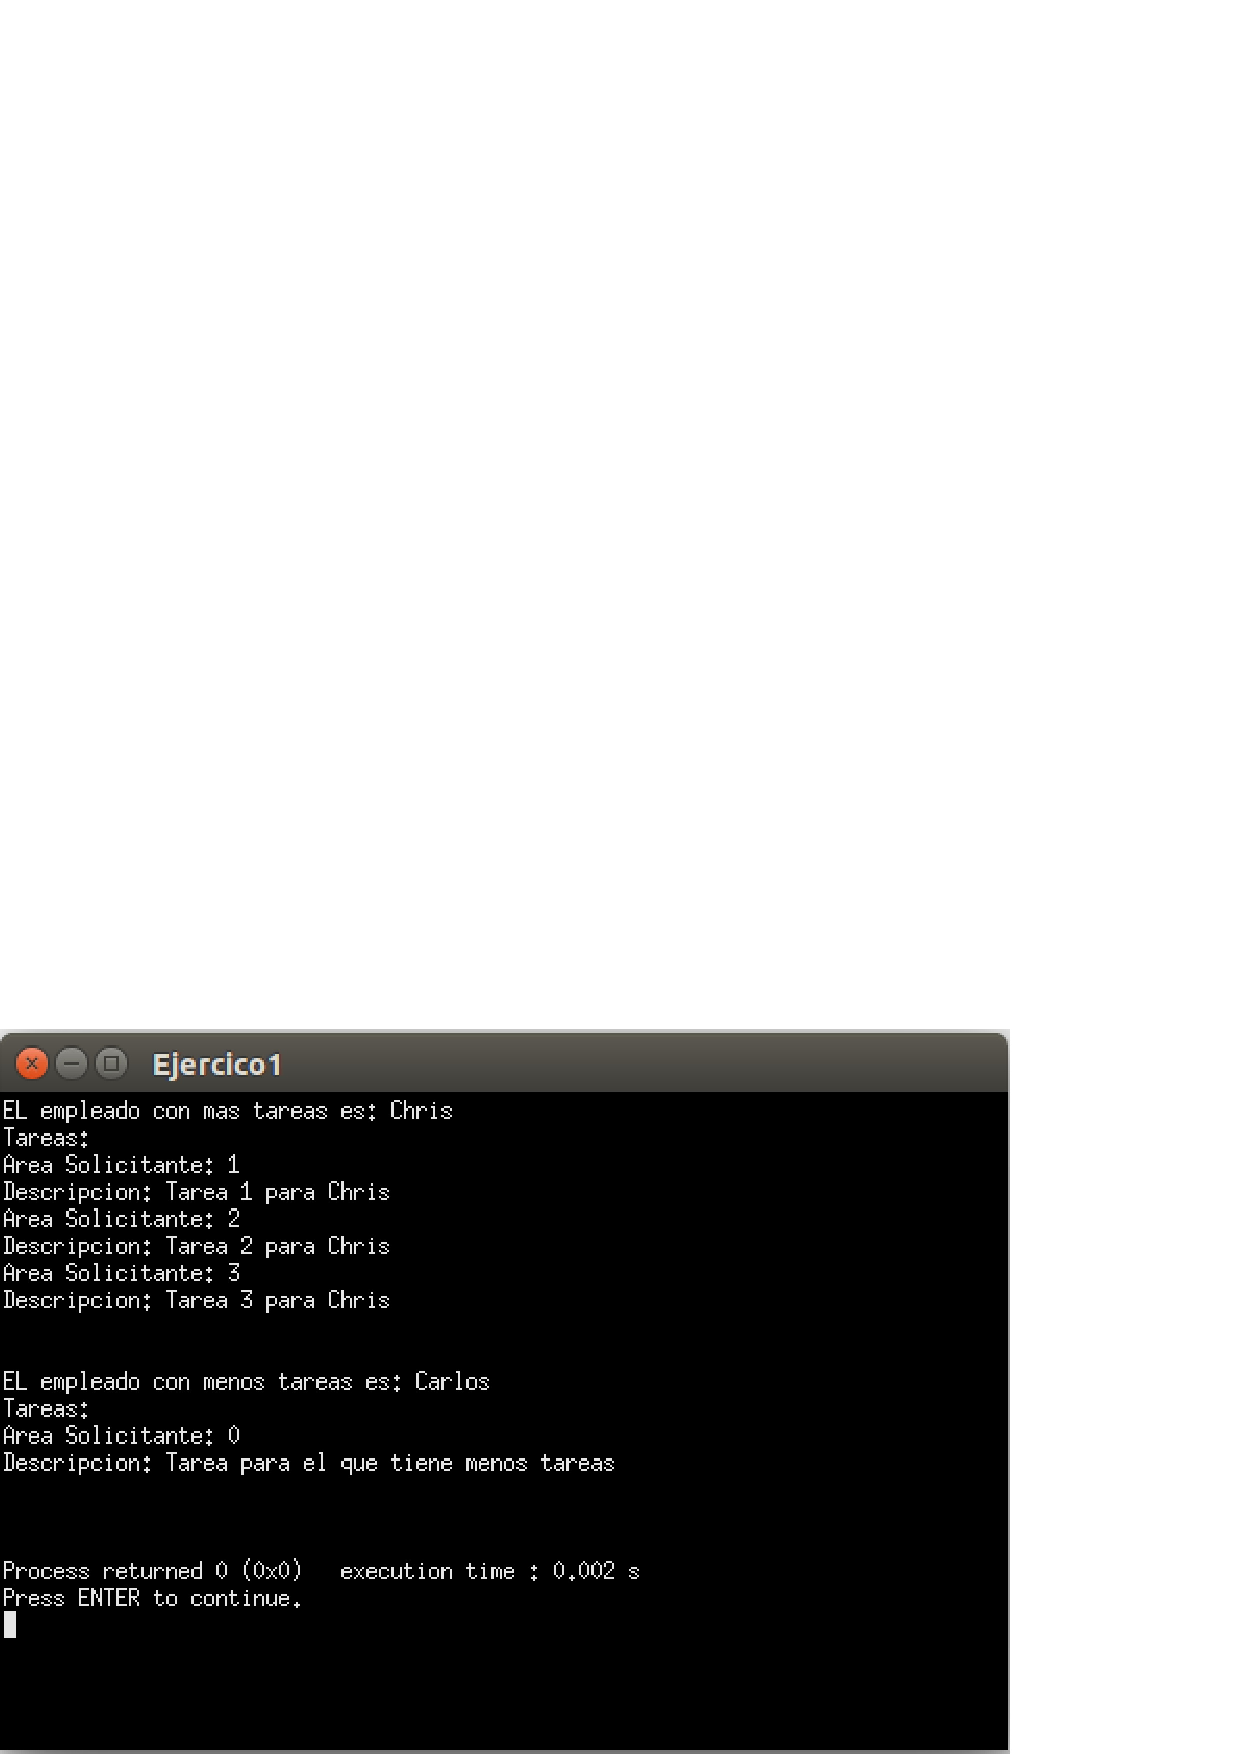
\includegraphics[scale = 0.4]{1.png}
 \caption{Resultados}
\end{figure}

\item \textbf{Probar el siguiente código que muestra los modos de dibujar un polígono}

\begin{figure}[H]
  \centering
  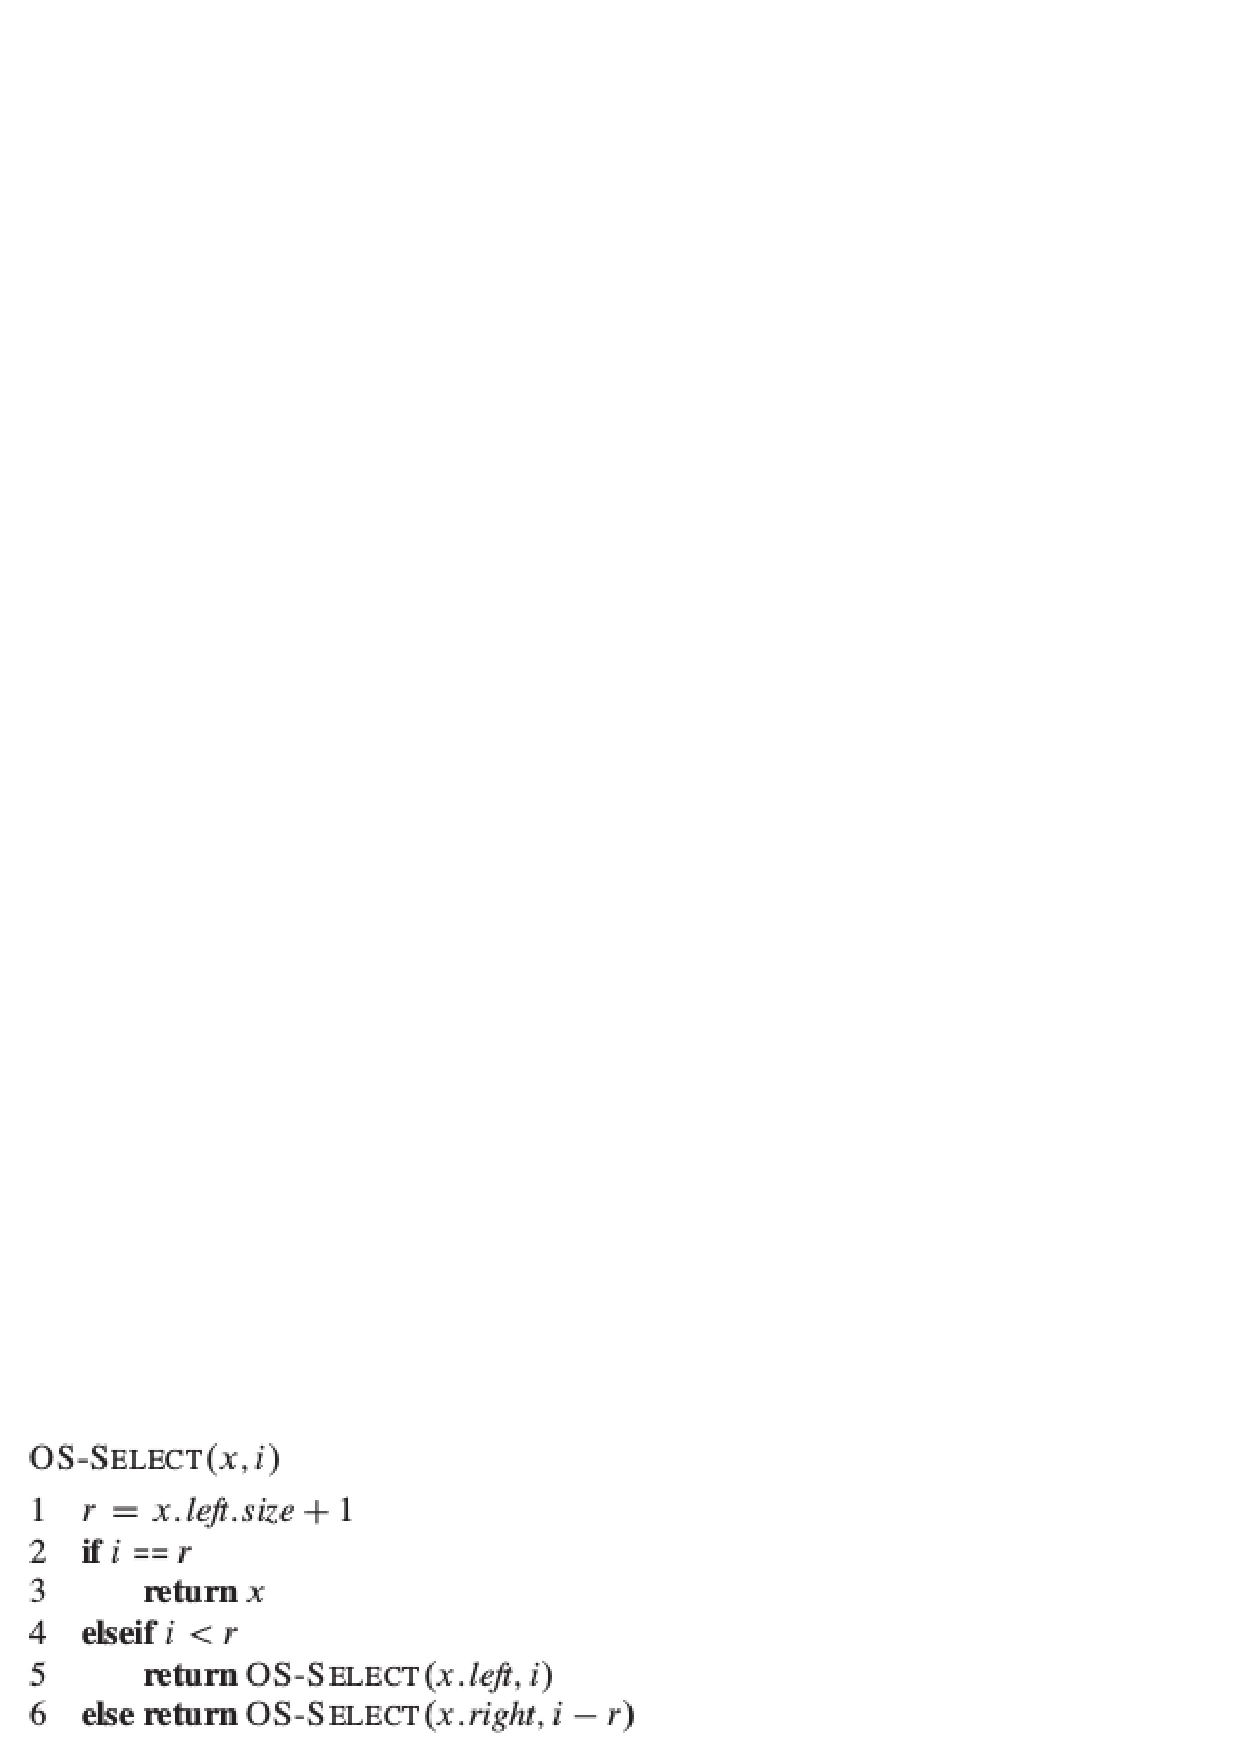
\includegraphics[scale = 0.5]{2.png}
  \caption{Resultados}
\end{figure}

\item \textbf{Dibuje los polígonos con colores interpolados ``glShadeModel(GL\_SMOOTH)''}

\begin{lstlisting}
#include <GL/glut.h>
#include <iostream>

using namespace std;

GLsizei winWidth = 800, winHeight = 600;


void init(void){
    glClearColor(1.0,1.0,1.0,1.0);
    glMatrixMode(GL_PROJECTION);
    gluOrtho2D(0.0, 800.0, 0.0, 600.0);
}

void display(){
	glClear(GL_COLOR_BUFFER_BIT);
	glColor3f(1.0, 0.0, 0.0);
	glShadeModel(GL_SMOOTH);
	glPolygonMode(GL_FRONT, GL_FILL);
	glBegin(GL_POLYGON);
		glVertex2i(10, 10);
		glVertex2i(100, 10);
		glColor3f(0.0, 1.0, 0.0);
		glVertex2i(150, 50);
		glVertex2i(100, 100);
		glColor3f(0.0, 0.0, 1.0);
		glVertex2i(50, 80);
		glVertex2i(10, 10);
	glEnd();
	glFlush();
}

int main(int argc, char **argv){
    glutInit(&argc, argv);
    glutInitDisplayMode(GLUT_SINGLE | GLUT_RGB);
    glutInitWindowSize(winWidth, winHeight);
    glutInitWindowPosition(100, 100);
    glutCreateWindow("Ejercicio 2");
    init();
    glutDisplayFunc(display);
    glutMainLoop();
    return 0;
}
\end{lstlisting}

\begin{figure}[H]
  \centering
  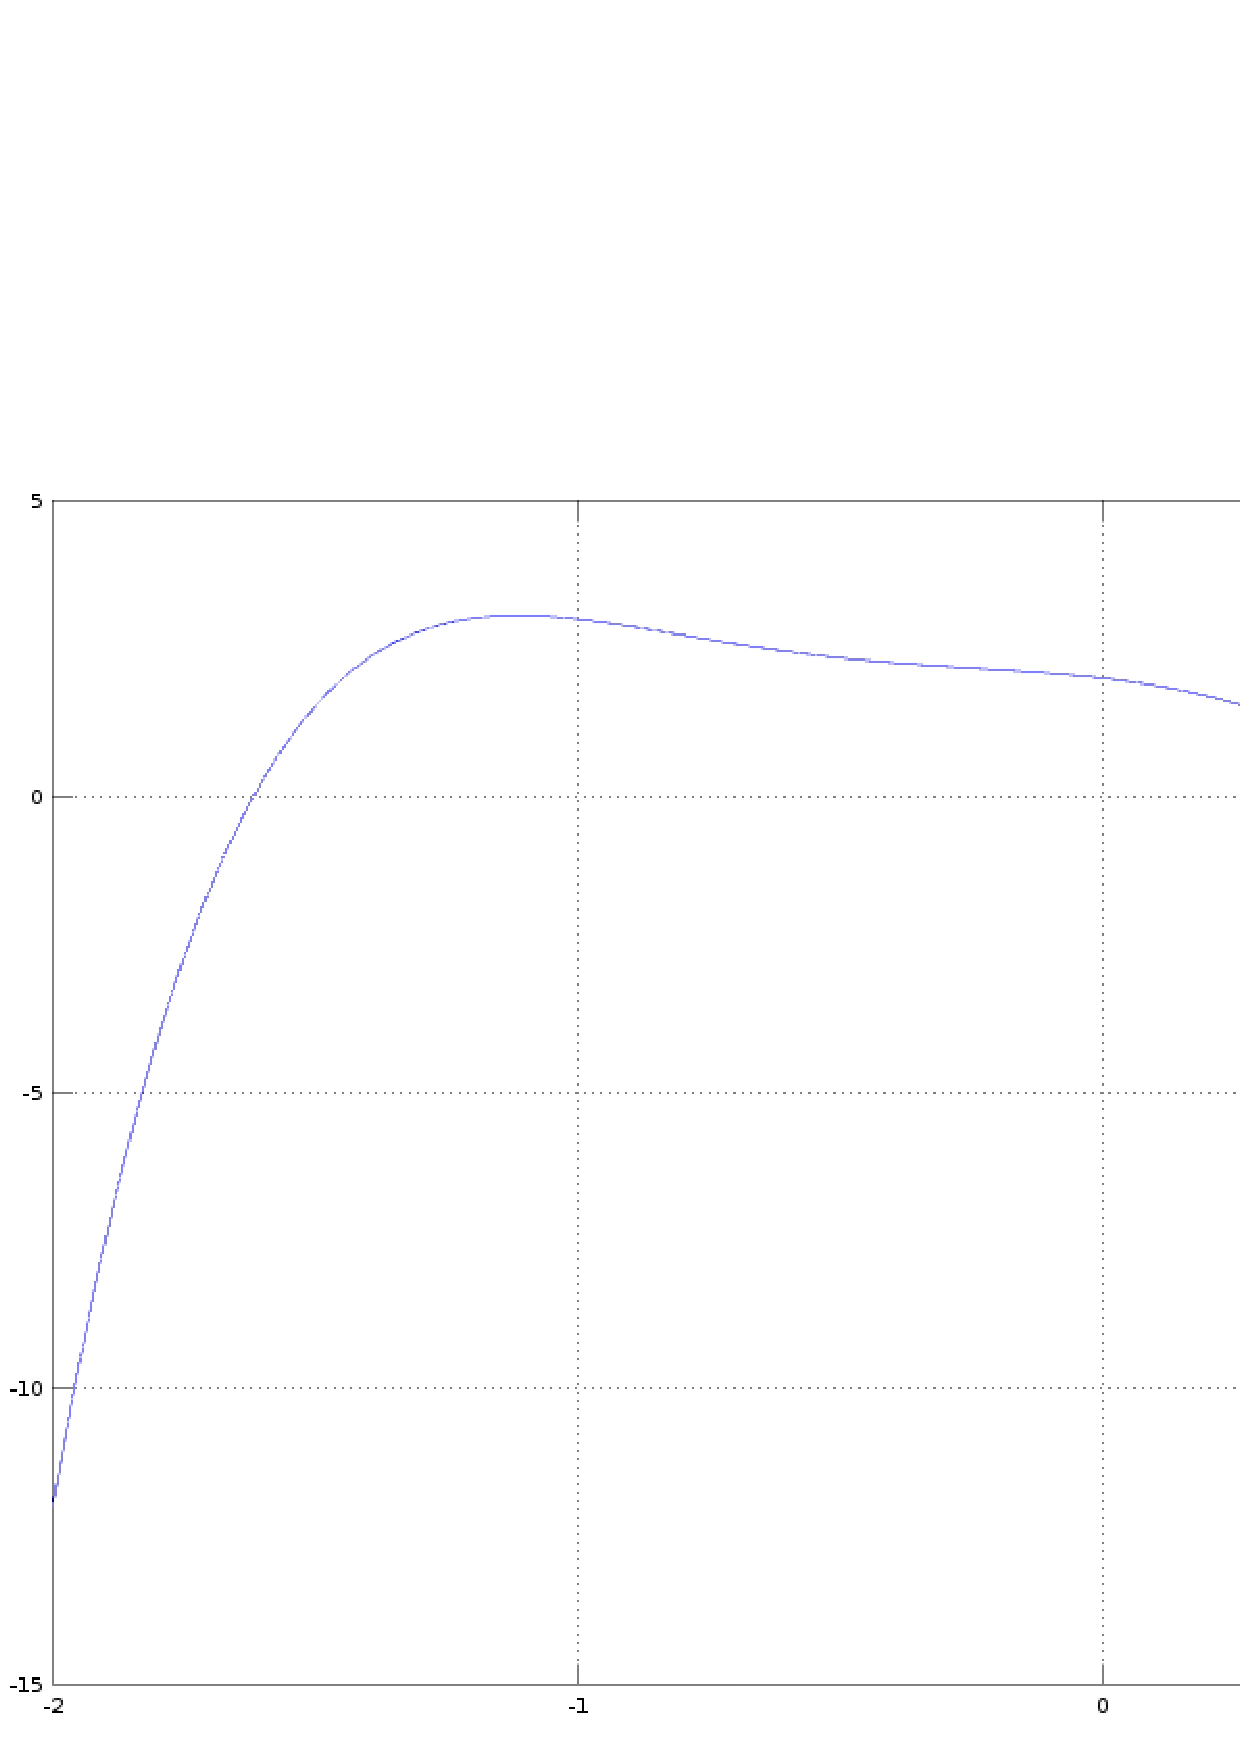
\includegraphics[scale = 0.5]{3.png}
  \caption{Resultados}
\end{figure}

\item \textbf{Probar el siguiente código que muestra un polígono con patrones}

\begin{figure}[H]
 \centering
 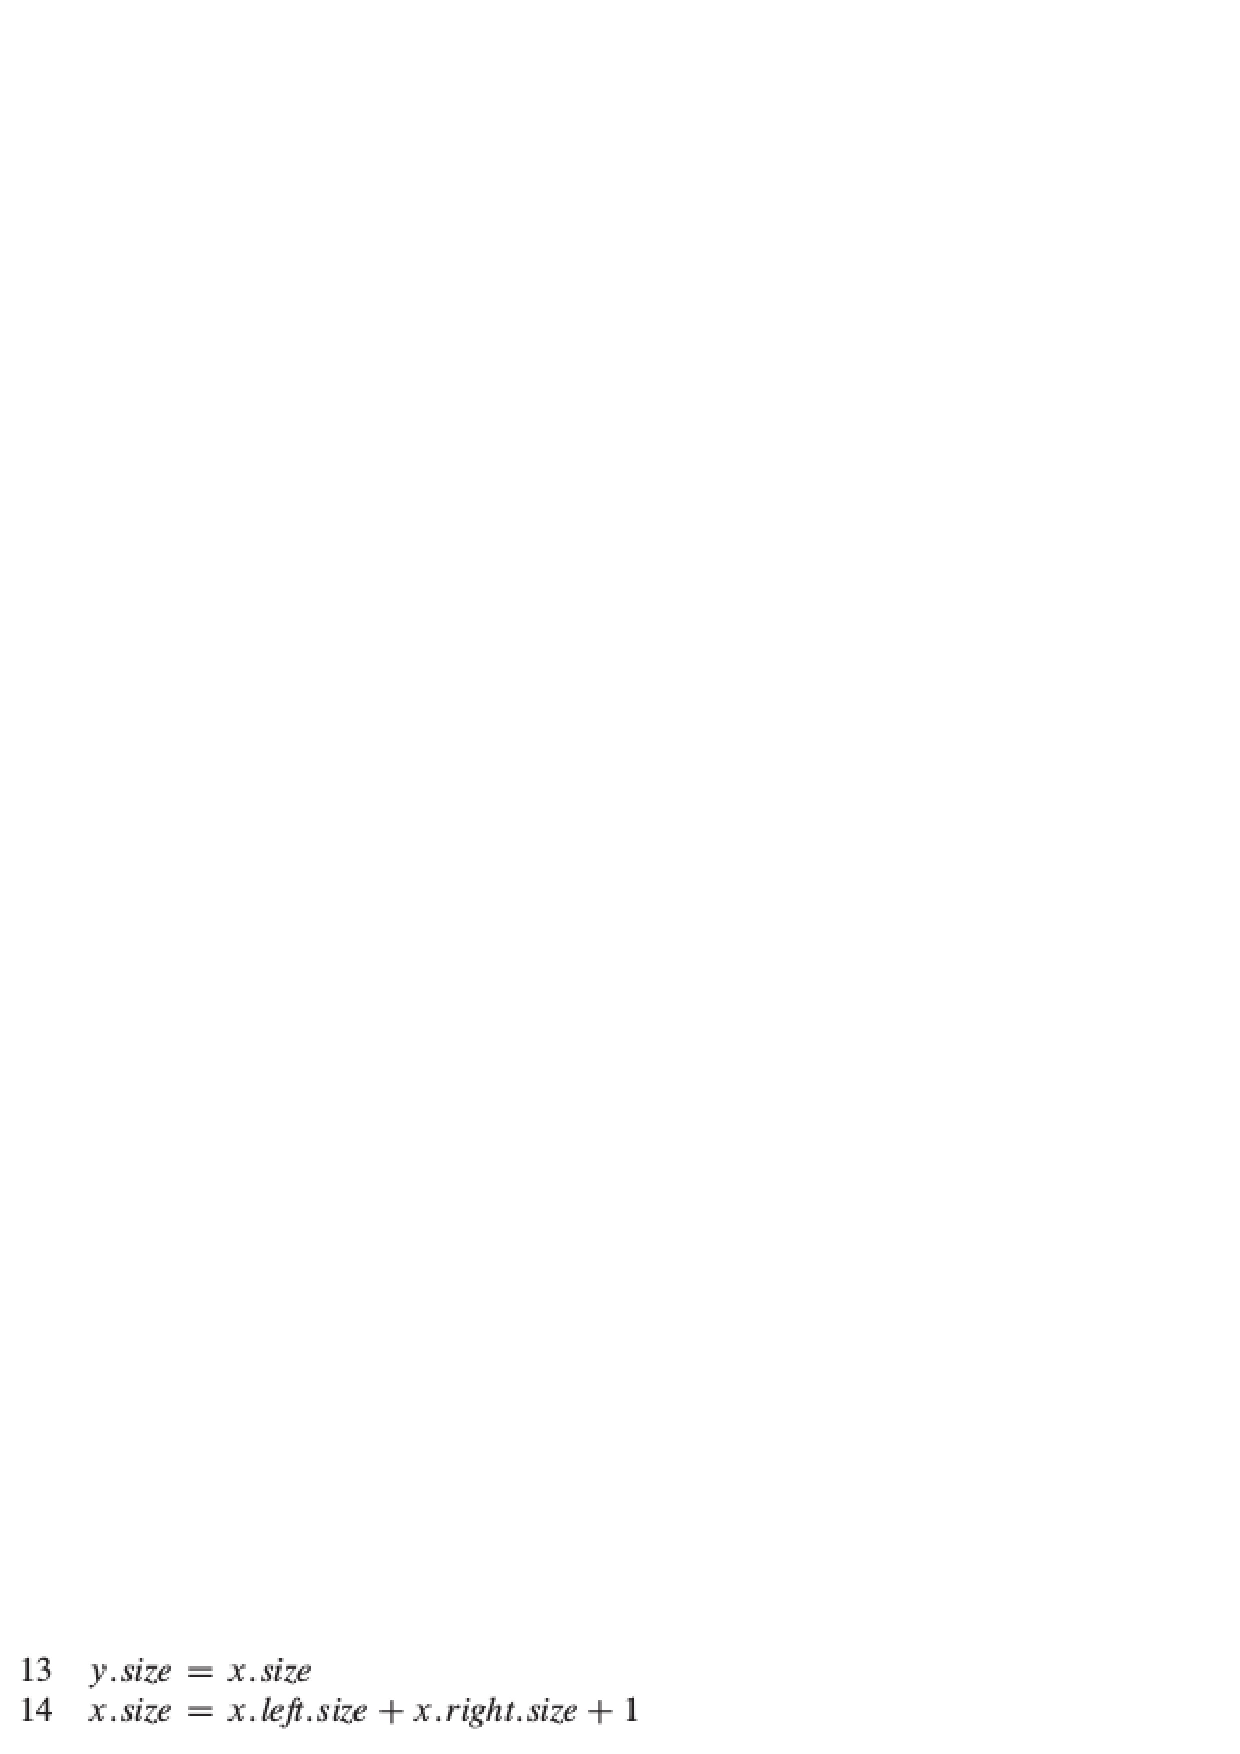
\includegraphics[scale = 0.5]{4.png}
 \caption{Resultados}
\end{figure}

\item \textbf{Realice un diseño artístico utilizando polígonos, aplicando patrones y colores}

\begin{lstlisting}
#include <GL/glut.h>
#include <iostream>
#include <tuple>
#include <cstdlib>
#include <ctime>

using namespace std;

GLsizei winWidth = 1200, winHeight = 800;
typedef tuple<float,float,float> Color;
enum COLORES {ROJO, VERDE, AZUL, BLANCO, NEGRO, GRIS_CLARO, CORAL, ORO, CELESTE, NARANJA, ROSADO, CELESTE2, VIOLETA, AMARILLO,
            CYAN, MAGENTA};

    GLubyte fly[] = {
        0x00, 0x00, 0x00, 0x00, 0x00, 0x00, 0x00, 0x00, 
        0x03, 0x80, 0x01, 0xc0, 0x06, 0xc0, 0x03, 0x60,
        0x04, 0x60, 0x06, 0x20, 0x04, 0x30, 0x0c, 0x20,
        0x04, 0x18, 0x18, 0x20, 0x04, 0x0c, 0x30, 0x20,
        0x04, 0x06, 0x60, 0x20, 0x44, 0x03, 0xc0, 0x22,
        0x44, 0x01, 0x80, 0x22, 0x44, 0x01, 0x80, 0x22,
        0x44, 0x01, 0x80, 0x22, 0x44, 0x01, 0x80, 0x22,
        0x44, 0x01, 0x80, 0x22, 0x44, 0x01, 0x80, 0x22,
        0x66, 0x01, 0x80, 0x66, 0x33, 0x01, 0x80, 0xcc,
        0x19, 0x81, 0x81, 0x98, 0x0c, 0xc1, 0x83, 0x30,
        0x07, 0xe1, 0x87, 0xe0, 0x03, 0x3f, 0xfc, 0xc0,
        0x06, 0x64, 0x26, 0x60, 0x0c, 0xcc, 0x33, 0x30,
        0x18, 0xcc, 0x33, 0x18, 0x10, 0xc4, 0x23, 0x08,
        0x10, 0x63, 0xc6, 0x08, 0x10, 0x30, 0x0c, 0x08,
        0x10, 0x18, 0x18, 0x08, 0x10, 0x00, 0x00, 0x08};

Color getColor(int color){
    switch(color){
        case ROJO: return make_tuple(1.0,0.0,0.0);
        case VERDE: return make_tuple(0.0,1.0,0.0);
        case AZUL: return make_tuple(0.0,1.0,0.0);
        case BLANCO: return make_tuple(1.0,1.0,1.0);
        case NEGRO: return make_tuple(0.0,0.0,0.0);
        case GRIS_CLARO: return make_tuple(0.658824,0.658824,0.658824);
        case CORAL: return make_tuple(1.0, 0.498039, 0.0);
        case ORO: return make_tuple(0.8, 0.498039, 0.196078);
        case CELESTE: return make_tuple(0.74902, 0.847059, 0.847059);
        case NARANJA: return make_tuple(1.0, 0.5, 0.0);
        case ROSADO: return make_tuple(0.737255, 0.560784, 0.560784);
        case CELESTE2: return make_tuple(0.196078, 0.6, 0.8);
        case VIOLETA: return make_tuple(0.309804, 0.184314, 0.309804);
        case AMARILLO: return make_tuple(1.0,1.0,0.0);
        case CYAN: return make_tuple(0.0,1.0,1.0);
        case MAGENTA: return make_tuple(1.0,0.0,1.0);
    }
}

void init(void){
    glClearColor(1.0,1.0,1.0,1.0);
    glMatrixMode(GL_PROJECTION);
    gluOrtho2D(0.0, 1200.0, 0.0, 800.0);
}

void drawString(string s, int x, int y){
	glColor3f(0.0, 0.0, 0.0);
	glRasterPos2i(x,y);
	for(char c : s){
		glutBitmapCharacter(GLUT_BITMAP_HELVETICA_12,c);
	}
	glColor3f(1.0, 0.0, 0.0);
}

void display(void){
	glClear(GL_COLOR_BUFFER_BIT);
    glColor3f(0.658824, 0.658824, 0.658824);
    int colX = 50;
    int colY = 600;
    int piso = 50;

    glBegin(GL_QUAD_STRIP);
        glVertex2i(colX, colY);
        glVertex2i(colX + 100, colY);
        glVertex2i(colX + 20, colY - 50);
        glVertex2i(colX + 80, colY - 50);
        glVertex2i(colX + 20, colY - (colY - 100));
        glVertex2i(colX + 80, colY - (colY - 100));
        glVertex2i(colX, piso);
        glVertex2i(colX + 100, piso);
    glEnd();

    glFlush();

    glColor3f(0.0 ,0.0, 0.0);
    glEnable(GL_POLYGON_STIPPLE);
    glPolygonStipple(fly);
    glBegin(GL_QUAD_STRIP);
        glVertex2i(colX, colY);
        glVertex2i(colX + 100, colY);
        glVertex2i(colX + 20, colY - 50);
        glVertex2i(colX + 80, colY - 50);
        glVertex2i(colX + 20, colY - (colY - 100));
        glVertex2i(colX + 80, colY - (colY - 100));
        glVertex2i(colX, piso);
        glVertex2i(colX + 100, piso);
    glEnd();
    glDisable(GL_POLYGON_STIPPLE);
    glColor3f(0.658824, 0.658824, 0.658824);
    colX = 1050;
    
    glBegin(GL_QUAD_STRIP);
        glVertex2i(colX, colY);
        glVertex2i(colX + 100, colY);
        glVertex2i(colX + 20, colY - 50);
        glVertex2i(colX + 80, colY - 50);
        glVertex2i(colX + 20, colY - (colY - 100));
        glVertex2i(colX + 80, colY - (colY - 100));
        glVertex2i(colX, piso);
        glVertex2i(colX + 100, piso);
    glEnd();

    glColor3f(0.0 ,0.0, 0.0);
    glEnable(GL_POLYGON_STIPPLE);
    glPolygonStipple(fly);
    glBegin(GL_QUAD_STRIP);
        glVertex2i(colX, colY);
        glVertex2i(colX + 100, colY);
        glVertex2i(colX + 20, colY - 50);
        glVertex2i(colX + 80, colY - 50);
        glVertex2i(colX + 20, colY - (colY - 100));
        glVertex2i(colX + 80, colY - (colY - 100));
        glVertex2i(colX, piso);
        glVertex2i(colX + 100, piso);
    glEnd();
    glDisable(GL_POLYGON_STIPPLE);

    glColor3f(0.658824, 0.658824, 0.658824);
    glBegin(GL_TRIANGLES);
        glVertex2i(50, colY);
        glVertex2i(600, 800);
        glVertex2i(1150, colY);
    glEnd();

    glColor3f(0.0 ,0.0, 0.0);
    glEnable(GL_POLYGON_STIPPLE);
    glPolygonStipple(fly);
    glBegin(GL_TRIANGLES);
        glVertex2i(50, colY);
        glVertex2i(600, 800);
        glVertex2i(1150, colY);
    glEnd();
    glDisable(GL_POLYGON_STIPPLE);

    glColor3f(1.0,1.0,1.0);
    glBegin(GL_POLYGON);
        glVertex2i(600, 750);
        glVertex2i(550, 700);
        glVertex2i(600, 650);
        glVertex2i(650, 700);
    glEnd();

    glColor3f(0.0,0.0,0.0);
    glBegin(GL_POLYGON);
        glVertex2i(600, 720);
        glVertex2i(570, 700);
        glVertex2i(600, 680);
        glVertex2i(630, 700);
    glEnd();

    glPointSize(3);
    glColor3f(1.0,1.0,1.0);
    glBegin(GL_POINTS);
        glVertex2i(600, 700);
    glEnd();

    int limiteIzq = 150;
    int limiteDer = 1050;
    int limiteArr = colY;
    int limiteAbj = 50;
    int espacioX = limiteDer - limiteIzq;
    int espacioY = limiteArr - limiteAbj;
    
    int numeroPuntos = 20;
    int puntoX, puntoY;
    int color;
    float R, G, B;

    glColor3f(0.0,0.0,0.0);
    glBegin(GL_LINE_LOOP);
        glVertex2i(limiteIzq, limiteAbj);
        glVertex2i(limiteIzq, limiteArr);
        glVertex2i(limiteDer, limiteArr);
        glVertex2i(limiteDer, limiteAbj);
    glEnd();


    glBegin(GL_QUAD_STRIP);
    glVertex2i(limiteIzq, limiteArr);
    glVertex2i(limiteDer, limiteArr);
    for(int i = 0; i < numeroPuntos; i++){
        for(int j = 0; j < 2; j++){
            puntoX = rand() % espacioX + limiteIzq;
            puntoY = rand() % espacioY + limiteAbj;
            color = rand() % (MAGENTA + 1);
            tie(R, G, B) = getColor(color);
            glColor3f(R,G,B);
            glVertex2i(puntoX, puntoY);
        }
    }
    glVertex2i(limiteIzq, limiteAbj);
    glVertex2i(limiteDer, limiteAbj);
    glEnd();


    glFlush();
}


int main(int argc, char **argv){
    srand (time(NULL));
    glutInit(&argc, argv);
    glutInitDisplayMode(GLUT_SINGLE | GLUT_RGB);
    glutInitWindowSize(winWidth, winHeight);
    glutInitWindowPosition(100, 100);
    glutCreateWindow("Programa Primitivas");
    init();
    glutDisplayFunc(display);


    glutMainLoop();
    return 0;
}
\end{lstlisting}

\begin{figure}[H]
 \centering
 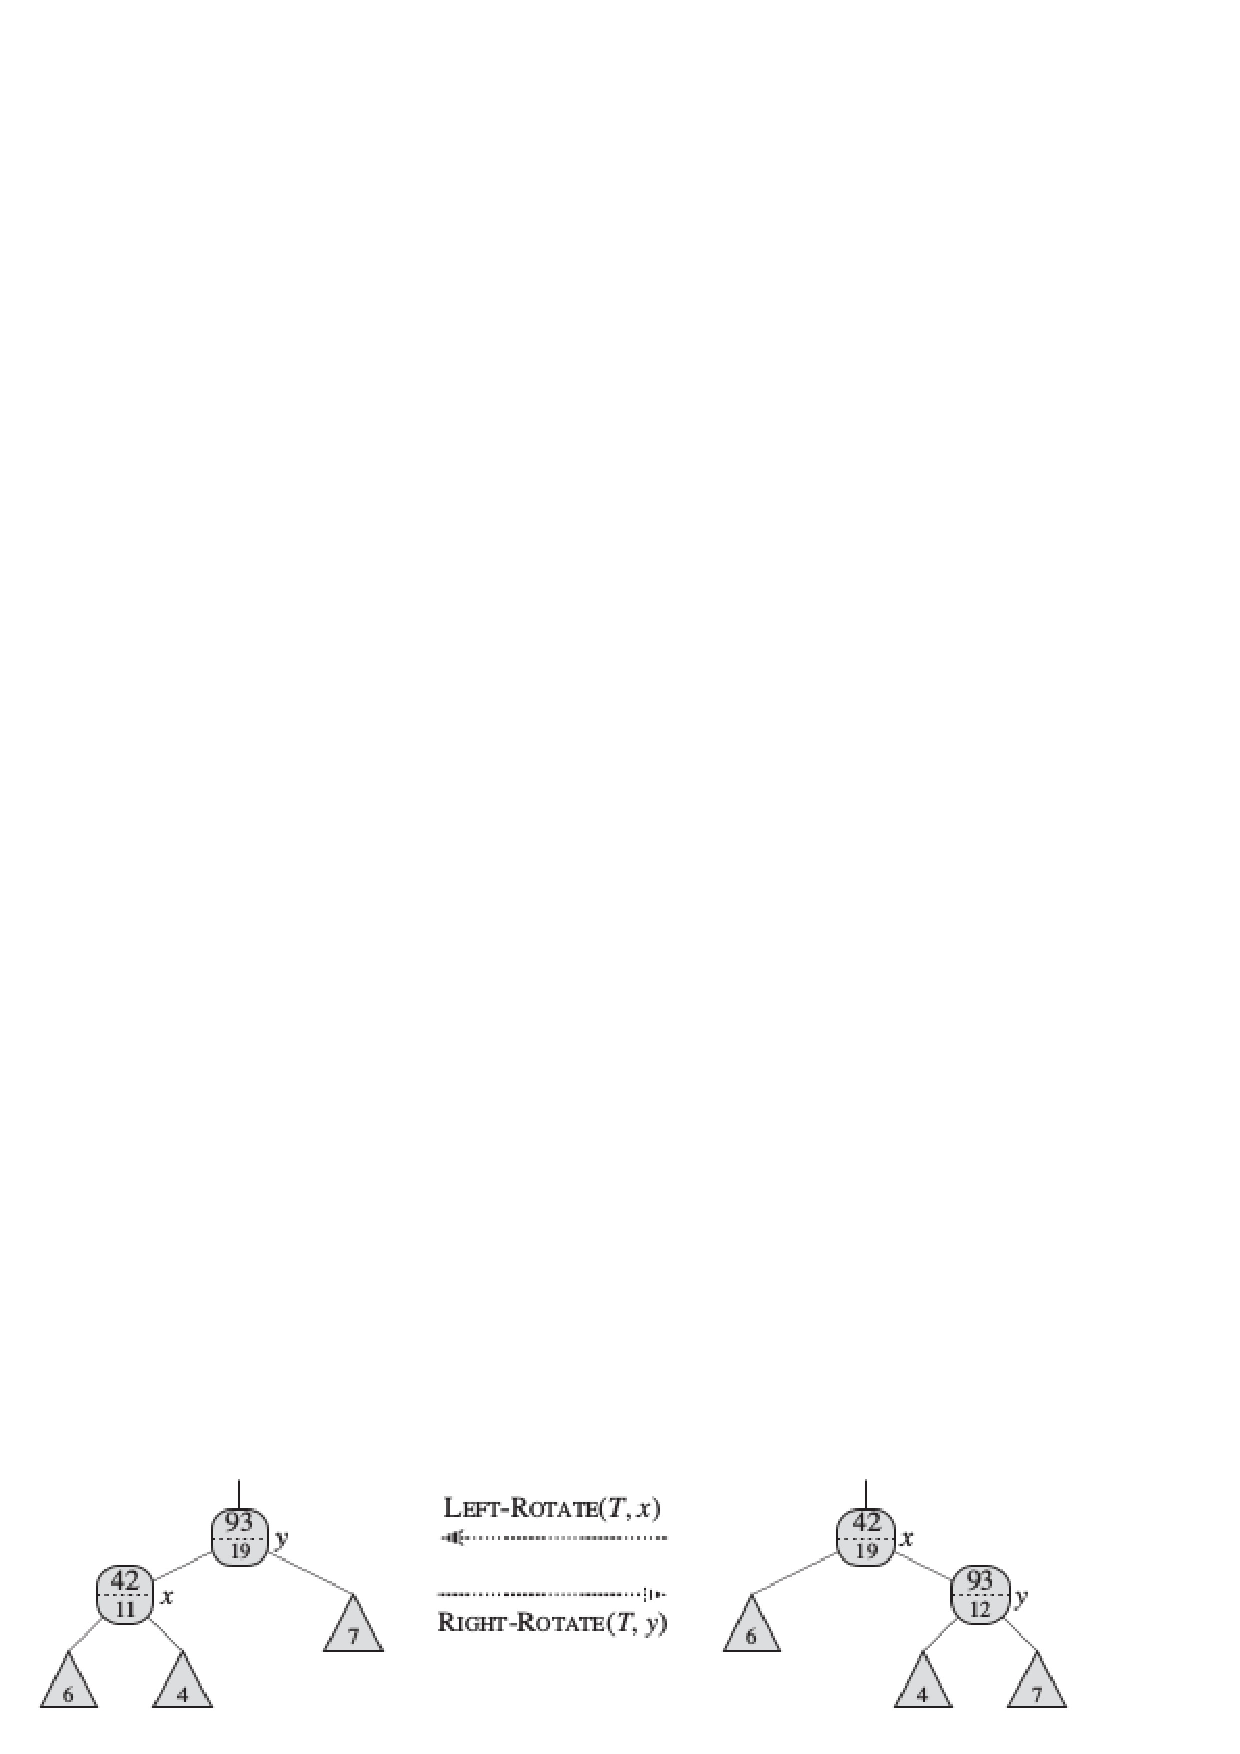
\includegraphics[scale = 0.35]{5.png}
 \caption{Resultados}
\end{figure}


\end{enumerate}

\end{document}

